\documentclass{tex/cls/eadmatUFRB}

\printanswers % <--------- Mostra as Soluções.

%=======================================
% Informações do Título da Lista
%=======================================
\tituloDaLista{Modelo Genérico} %---------> Coloque aqui o título da sua lista
\aluno{Fulano de Tal, Cicrano Beltrano} %-> Coloque aqui seu nome ou o nome do grupo (abreviar, se necessário)
\dataDia{00} %----------------------------> Dia de entrega da Atividade Avaliativa
\dataMes{00} %----------------------------> Mês de entrega da Atividade Avaliativa
\numeroDaLista{X} %-----------------------> Número da Lisda de Atividade (colocar números em algarismos romanos)
%=======================================

% Comandos simplificados ======================================================

%    \intc   ----> integral em curva fechada no sentido anti-horário.
%    \vazio  ----> conjunto vazio
%    \dd     ----> letra `d`  no modo romano (para usar em `dx' na integral)
%    \sen    ----> seno
%    \tg     ----> tangente
%    \arctg  ----> arcotangente
%    \Ln     ----> logarítmo maiúsculo
%    \Arg    ----> argumento maiúsculo
%    \Cis    ----> ('C' maiúsculo) abreveação para cos(x) +isen(x)
%    \cis    ----> ('c' minúsculo) abreveação para cis(x) 
%==============================================================================

%%%%%%%%%%%%%%%%%%%%%%%%%%%%%%%%%%%%%%%%%%%%%%%%%%%%%%%%%%%%%%%%%%%%%%%%%%%%%%%
% Início do Documento
%%%%%%%%%%%%%%%%%%%%%%%%%%%%%%%%%%%%%%%%%%%%%%%%%%%%%%%%%%%%%%%%%%%%%%%%%%%%%%%
\begin{document}
%
 \titulo %-------> Comando para gerar o cabeçalho estilizado (com logo da UFRB). 
%                  Não apagar esse comando!
 \begin{questions} %------> Ambiente para Questões (INÍCIO)
  %
   %==============================================================================
% Questão 01
%==============================================================================
\question[3] Considere o conjunto de pontos complexos
\[
		z(t) = (3 + 2 \cos{t}) + (-1 + 3 \sen{t})\,i,
\]
onde $ t \in \mathbb{R} $.
\begin{parts}
  \part[1] Mostre que $ \left| z^{n}(t) \right| = \left| z(t) \right|^{n} $,
	  para todo $ n \in \mathbb{N} $.
   %
    \begin{solution}
  Usaremos indução sobre $n$.
		É natural pensarmos: existe algum natural que essa igualdade seja 
		verdadeira?
		Bom\ldots não é difícil perceber que para $n=1$ ela é verdadeira.
		Para $n=2$ também é verdadeira\ldots
		Então, passamos a pensar: ``Talvez só existe algum subconjunto de 
		$ \mathbb{N} $ onde ela vale, mas não deve valer para todos os naturais''.
	 Seja, então, $ \mathcal{X} \subset \mathbb{N} $ definido por
	 \[
	  \mathcal{X} = 
		 \left\{\,
		 n \in \mathbb{N};\;\; \left| z^{n}(t) \right| = \left| z(t) \right|^{n}
		 \,\right\}
	 \]
	 ou seja, um subconjunto de número naturais onde se verifica a igualdade.
	 \begin{enumerate}
	  \item[(i)] $ 1 \in \mathcal{X} $; pois 
		  $
			  \left| z^{1}(t) \right| = 
			  \left| z(t) \right| =
			  \left| z(t) \right|^{1}
	 		$.
		 \item[(ii)] Além disso, se certo natural $ k \in \mathcal{X} $, então 
		  \[
			  \left| z^{k + 1}(t) \right| = 
		 	 \left| z^{k}(t) \cdot z(t) \right| =
				 \left| z^{k}(t) \right| \cdot \left| z(t) \right| = 
				 \left| z(t) \right|^{k} \cdot \left| z(t) \right| =
				 \left| z(t) \right|^{k + 1}
				\]
		  ou seja, ${k+1}\in\mathcal{X}$
	 \end{enumerate}
	 Ora, se o natural $ 1 $ está em $ \mathcal{X} $ e se para cada natural 
		$ k $ em $ \mathcal{X} $ o seu sucessor também está\ldots pelo Axioma~4
		de Peano, tem-se $ \mathcal{X} = \mathbb{N} $. Isso significa que a 
		igualdade não apenas é válida para uma parte dos naturais, mas para todo
		natural $ n $.
\end{solution}
   %
	 \part[0.5] Calcule o valor de $ \left| z^{4}(t) \right| $, quando 
		 $ t = 3 \pi / 2 $.
   %--------------------------------------------------------------------------- 
    \begin{solution} %--> Não esquecer do ambiente apropriado para as soluções!
	    Note que 
	    \[
	     z(3 \pi / 2) = 
		   	\left[ 3 + 2 \cos{(3 \pi / 2)} \right] + 
		   	\left[-1 + 3 \sen{(3 \pi / 2)} \right]\,i =
		   	(3 + 2 \cdot 0) + [-1 + 3 \cdot (-1)]\,i =
		   	3-4\,i.
	    \]
	    Ora, pelo item~(a), podemos fazer:
	    \[
	     \left| z^{4}(3 \pi / 2) \right| = 
		   	\left| z(3 \pi / 2) \right|^4 =
		   	\left| 3 - 4\,i \right|^4 = 
		   	\left( \sqrt{3^2 + (-4)^2} \right)^4 =
		   	25^2 =
		   	\Ovalbox{$625$}.
	    \]
    \end{solution}
   %---------------------------------------------------------------------------
	 \part[0.5] O que representa, geometricamente, esse conjunto de números 
		 complexos?
   %
    \begin{solution}
	 Seja $ z = x + y\,i $.
	 Fazendo $ x = 3 + 2 \cos{t} $ e $ y = -1 + 3 \sen{t} $, temos
	 \begin{align}
	  \cos{t} &= \frac{x - 3}{2} \label{cos}\\
	  \sen{t} &= \frac{y + 1}{3} \label{sen}
	 \end{align}
	 Elevado ao quadrado as equações \eqref{cos} e \eqref{sen}, e somando 
		membro a membro, encontramos:
	 \[
			\left( \frac{x - 3}{2} \right)^2 + \left (\frac{y + 1}{3} \right)^2 =
			\cos^{2}{t} + \sen^{2}{t}
			\Longrightarrow
			\Ovalbox{$\displaystyle\frac{(x-3)^2}{2^2}+\frac{(y-(-1))^2}{3^2}=1$}
		\]
  Ou seja, uma \emph{Elipse} de centro $ (3, -1) $ e de semieixos $ a = 2 $
		e $b=3$.
	 Veja a Figura~\ref{fig:elipse}.
  
  \begin{minipage}{\textwidth}
	  \centering
	  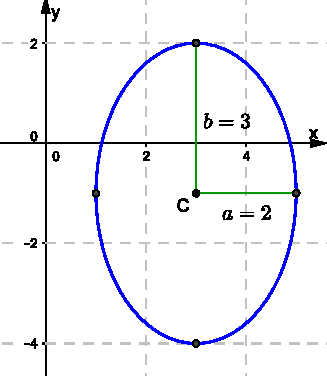
\includegraphics[width=5cm]{elipse}
	  \captionof{figure}{Conjunto dos complexos $z(t)$ visto geometricamente.}
	  \label{fig:elipse}
	 \end{minipage}  
\end{solution}
   %
\end{parts}
%==============================================================================
 %-------------------------------> Questão 01
   %\input{tex/questoes/02_questao} %-------------------------------> Questão 02
   %\input{tex/questoes/03_questao} %-------------------------------> Questão 03
  %
 \end{questions} %--------> Ambiente para Questões (TÉRMINO)
%
\end{document}
%%%%%%%%%%%%%%%%%%%%%%%%%%%%%%%%%%%%%%%%%%%%%%%%%%%%%%%%%%%%%%%%%%%%%%%%%%%%%%%